\documentclass[a4paper,11pt]{article}
\usepackage{amsmath}
\usepackage{graphicx}
\usepackage{caption}
\usepackage{amssymb}
\usepackage{verbatim}
\usepackage{hyperref}
\usepackage{listings}
\usepackage{float}
\usepackage[thinc]{esdiff}
\usepackage{euscript}
\usepackage{subcaption}
\usepackage{enumitem}
\usepackage{commath}
\setlength{\parindent}{0em}
\newcommand*{\field}[1]{\mathbb{#1}}%
\usepackage{amsthm}
\newtheorem{claim}{Claim}
\captionsetup{labelformat=empty}
\usepackage[nottoc]{tocbibind}
\usepackage{adjustbox}



\begin{document}
\lstset{language = Matlab}
\begin{titlepage} % Suppresses displaying the page number on the title page and the subsequent page counts as page 1
	
	\center % Centre everything on the page
	
	\vspace*{3cm}

	\textsc{Mathematical Tripos, Part II}\\
	\textsc{Computational project}
	\begin{center}
      {\huge\bfseries Parabolic Partial Differential Equations\\[0.4cm]
}     \end{center}
	
	\vfill
	\vfill\vfill\vfill\vfill
	\includegraphics*[width = 2.675cm, height = 3.1cm]{coat.png}
	\vfill
    \textsc{University of Cambridge}
	
	\vspace*{\fill}
	\vfill
	{\large\today} 
	\vfill
	
\end{titlepage}
\setcounter{tocdepth}{3}
\tableofcontents
\newpage
\section{Analytic Solution}
\subsection*{Question 1}
\begin{enumerate}[label = (\roman*)]
  \item 
  Write $\theta = f(t)(1-x)+\phi(x,t)$, and substitute into the diffusion equation, we have the following governing equation:
  $$2(3t-1)(1-x) + \phi_{t} = \phi_{xx}$$on the interval $0 \leqslant x \leqslant 1$, with boundary conditions:\\
  $$\phi(0,t) = \phi(1,t) = 0$$ for $0 \leqslant t \leqslant \infty$, and initial condition:
  $$\phi(x, t) = -(3t-2)t(1-x) $$ for $t\leqslant 0$, $0 \leqslant x \leqslant 1$.\\
  Write $\phi$ in a Fourier Sine Series in x: $\phi(x,t) = \sum_{n=1}^{\infty}g_{n}(t) \sin(n\pi x)$, and $1-x = \sum_{n=1}^{\infty}\frac{2}{n\pi}\sin(n \pi x)$
  Then we have:
  $$\frac{4}{n \pi}(3t-1)+ g'_{n} = -n^{2}\pi^{2} g_{n}$$
  for $n = 1,2,3 \cdots$ with initial condition:
$\phi(x, 0) = 0$ for $0 \leqslant x \leqslant 1$.\\
  and the solution is 
$$g_{n}(t) = \frac{4}{n^3 {\pi}^3} (1-3t) + \frac{12}{n^5 {\pi}^5} -\frac{4}{n^3 {\pi}^3}(1+\frac{3}{n^2 {\pi}^2})e^{-n^2 {\pi}^2 t}$$ 
for $t \geqslant 0$, $n = 1,2,3 \cdots$.
  \item
  Known that $$2\int_{0}^{1}x\sin(n\pi x) dx = 2\frac{(-1)^{n+1}}{n \pi}$$
   $$ 2\int_{0}^{1}x^2\sin(n\pi x) dx = \frac{4((-1)^{n} - 1)}{n^3 \pi^3} + 2\frac{(-1)^{n+1}}{n \pi}\
   $$
   $$ 2\int_{0}^{1}x^3\sin(n\pi x) dx = \frac{12(-1)^{n}}{n^3 \pi^3} +2\frac{(-1)^{n+1}}{n \pi}
   $$
   $$ 2\int_{0}^{1}x^4\sin(n\pi x) dx =  \frac{48(1-(-1)^{n})}{n^5 \pi^5} +\frac{24(-1)^{n}}{n^3 \pi^3} +2\frac{(-1)^{n+1}}{n \pi}
   $$
   $$ 2\int_{0}^{1}x^5\sin(n\pi x) dx =  (-\frac{240}{n^5 \pi^5}+\frac{40}{n^3 \pi^3} -\frac{2}{n \pi})(-1)^{n}
   $$
  From the Fourier Series Solution, as $t\to \infty$, $$g_{n}(t) \to -\frac{12}{n^3 \pi^3}t + \frac{4}{n^3 {\pi}^3}(1+\frac{3}{n^2 {\pi}^2})$$ and the functions are:
  $$ \alpha (x) = - \sum_{n=1}^{\infty} \frac{12}{n^3 \pi^3}\sin(n\pi x) = -(x^3 - 3x^2 +2x) $$
  $$= -x(x-2)(x-1)$$
 $$ \beta(x) = \sum_{n=1}^{\infty}  \frac{4}{n^3 {\pi}^3}(1+\frac{3}{n^2 {\pi}^2})\sin(n\pi x) = -\frac{x^5}{20} +\frac{x^4}{4}-x^2+\frac{4}{5}x$$
 $$= -\frac{1}{20}x(x-1)(x-2)(x+2)(x-4)$$
 \item 
 The programme is in \ref{P1}.
 \item
 Plot at times t = 0.1, 2/3 and 1 ,according to the initial condition $(3t-2)t$.
 \begin{figure}[H]
 \center
 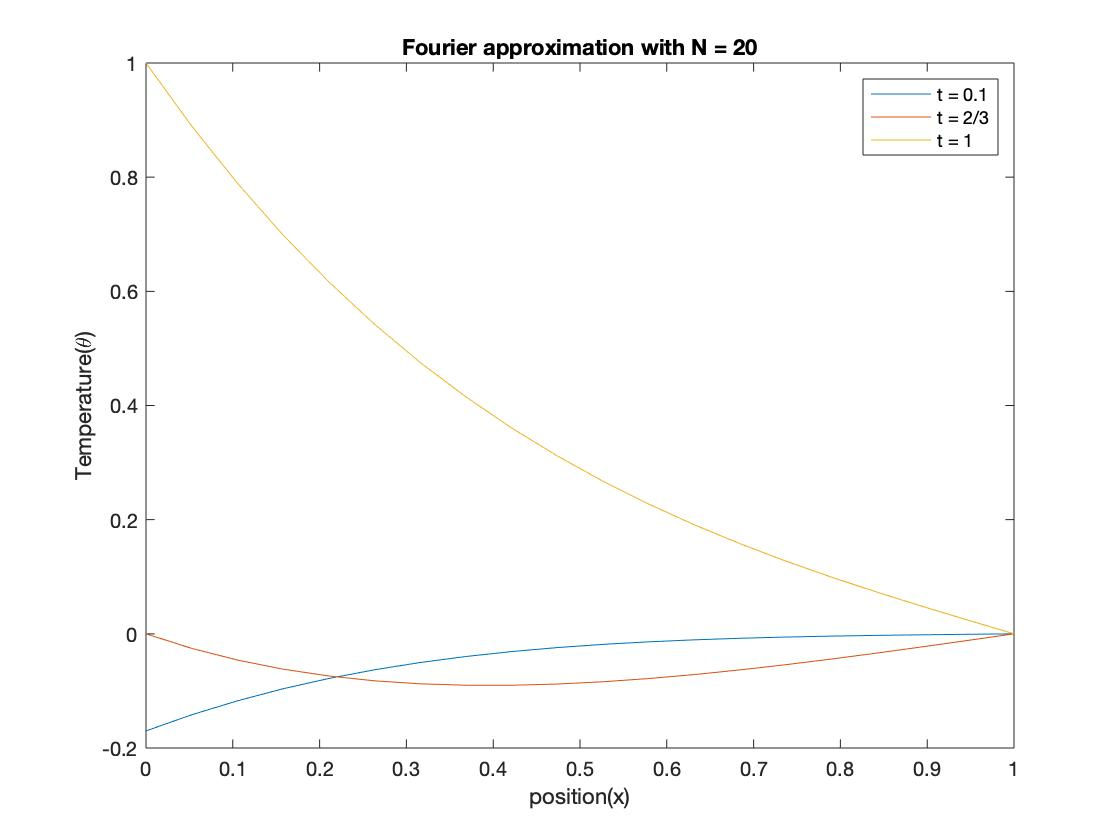
\includegraphics[width = 0.9\linewidth, height =8cm]{Q1.jpg}
 \caption{Figure 1.1: Fourier series solution at given times}
 \end{figure}
 \item
 The convergence is sufficiently accurate as we used a truncated sum of the first 6 terms. By using a Fourier Sine Series we actually extended $\phi$ to $-1\leqslant x \leqslant 1$, with $\phi$ odd, and computed its Fourier series. Since we have periodic boundary condition for $\phi$, and by knowledge from Numerical Analysis II the N point Fourier approximation of an analytic periodic function converges at spectral speed. i.e. the error is $O(N^{-p})$, for any $p = 1,2,3\cdots$.
 \item
 The evolution of temperature in space consists with the second law of Thermodynamics. The heat flows from the hot spot to the cold spot. By the Fourier law of heat conduction, the heat flux is proportional to the temperature difference when the length of material is fixed, i.e. we have $$q = -D\nabla \theta$$, where D is the diffusivity, which is a positive constant. The rate of change of the internal energy is proportional to that of the temperature by 
 $$\frac{\partial E}{ \partial t} = \rho c\frac{\partial \theta}{\partial t}$$ where $\rho$ is the density and $c$ is the specific heat capacitance. Both are positive constants. Then from conservation of energy and divergence theorem, after rescaling, we reach the diffusion equation as given. 
The time evolution is due to the initial condition at $x = 0$. When $t \leqslant \frac{2}{3}$, the hot spot is $x = 1$. Otherwise it is $x = 0$. So the direction of heat flow is right to left before  $t = \frac{2}{3}$ and is left to right after that. As time goes by, the left end is heated up and the temperature rises quadratically with time. But the temperature still drops fast close to the right end.
\end{enumerate}
\section{Numerical Methods}
\subsection*{Question 2}
\begin{enumerate}[label = (\roman*)]
 \item
 On next page. $v = 1/2$ in each case.
 \newpage
\begin{figure}[H]
\begin{subfigure}{0.5\textwidth}
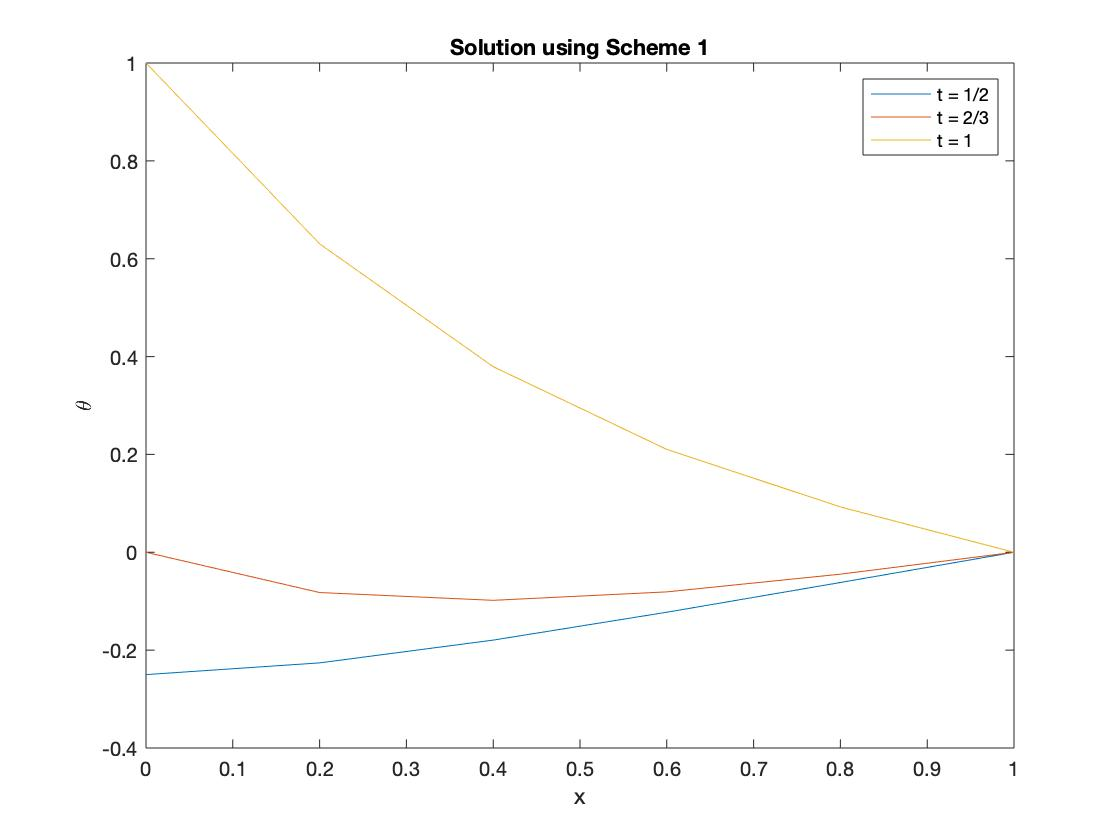
\includegraphics[width = \linewidth, height = 5cm]{Q2(1).jpg}
\caption{Figure 2.1: numerical solutions with scheme 1 at given times}
\label{Q2(1)}
\end{subfigure}
\begin{subfigure}{0.5\textwidth}
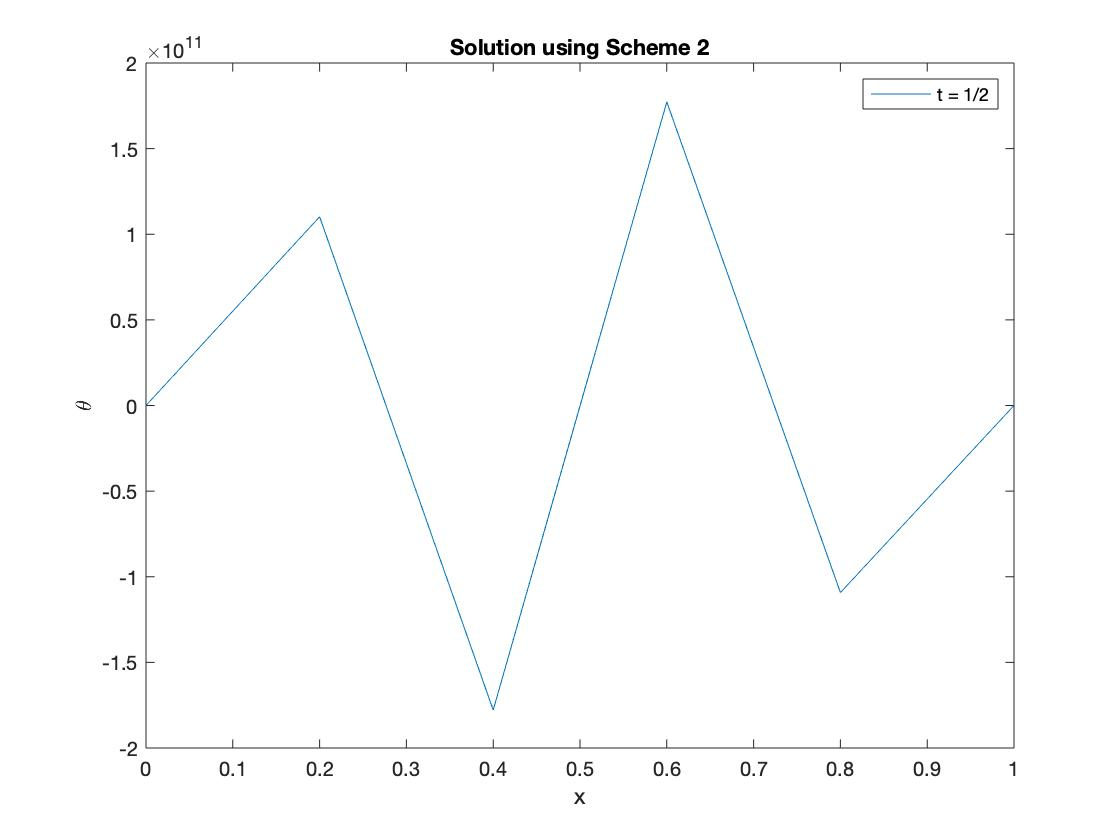
\includegraphics[width = \linewidth, height = 5cm]{Q2(2).jpg}
\caption{Figure 2.2: numerical solutions with scheme 2 at given times}
\label{Q2(2)}
\end{subfigure}
\begin{subfigure}{0.5\textwidth}
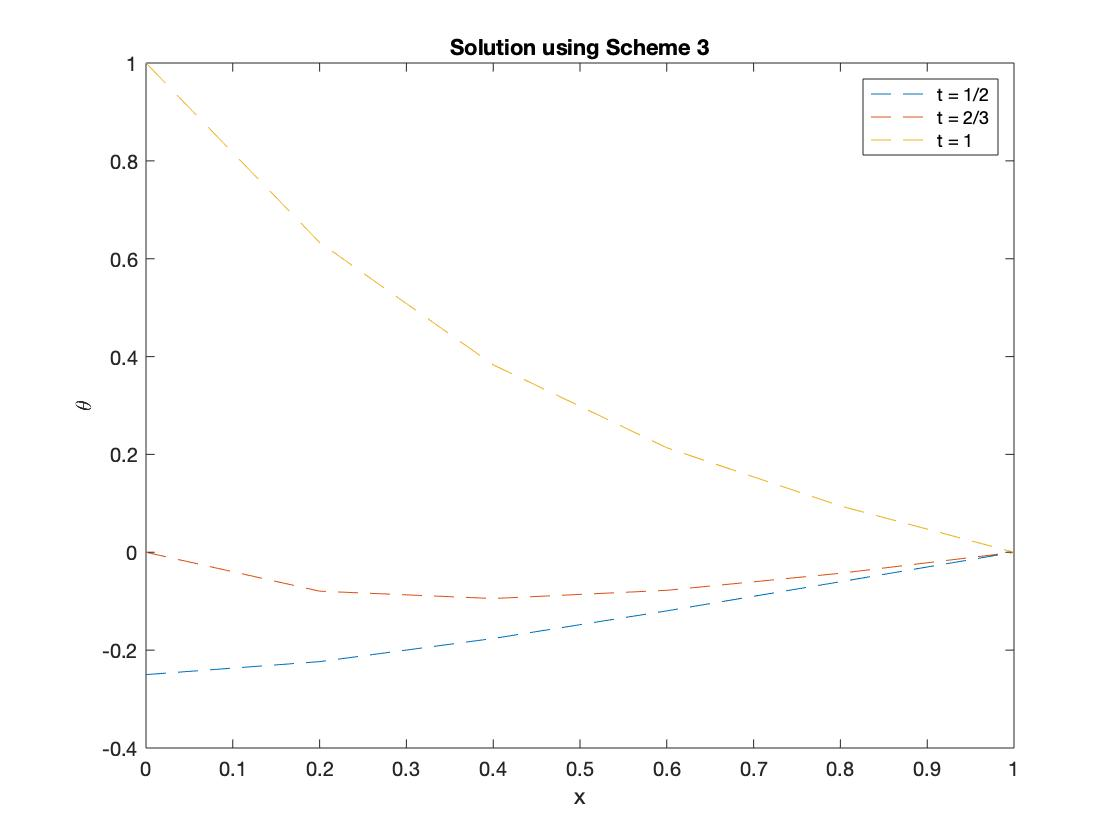
\includegraphics[width = \linewidth, height = 5cm]{Q2(3).jpg}
\caption{Figure 2.3: numerical solutions with scheme 3 at given times}
\label{Q2(3)}
\end{subfigure}
\begin{subfigure}{0.5\textwidth}
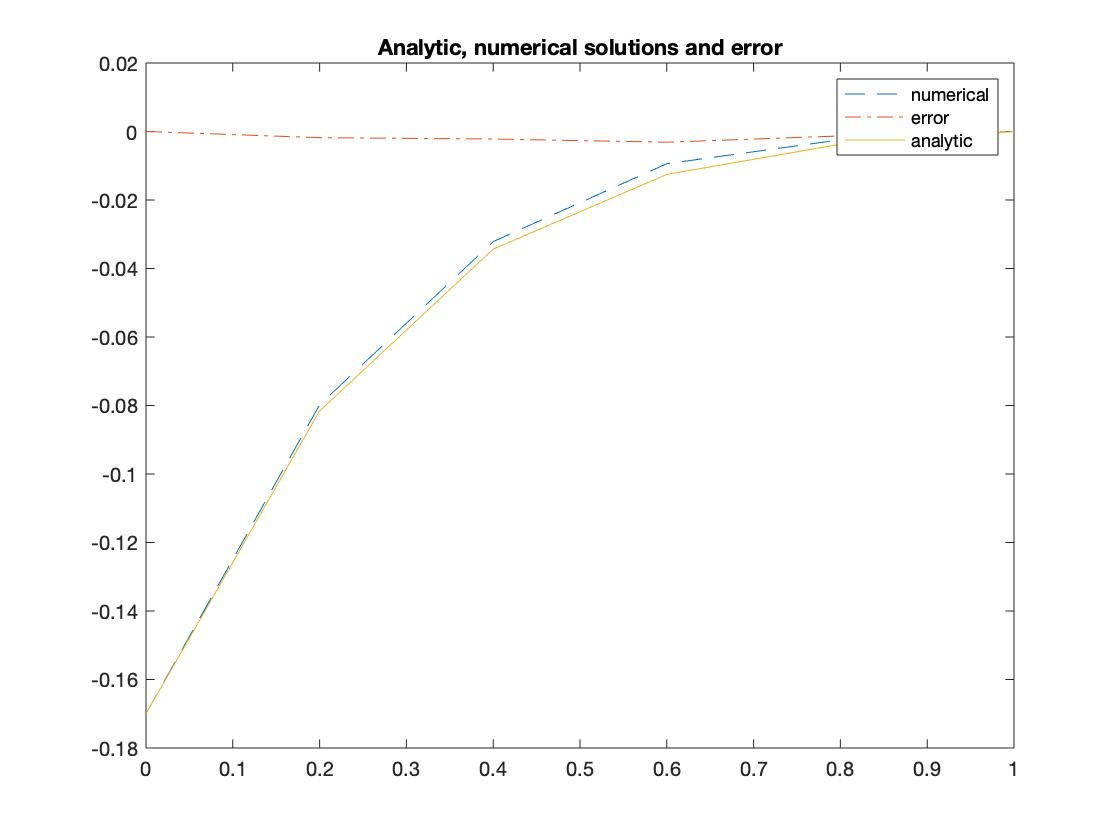
\includegraphics[width = \linewidth, height = 5cm]{Q2(4).jpg}
\caption{Figure 2.4: Analytic, numerical solution and error of scheme 1 at t = 0.1 }
\label{Q2(4)}
\end{subfigure}
\begin{subfigure}{0.5\textwidth}
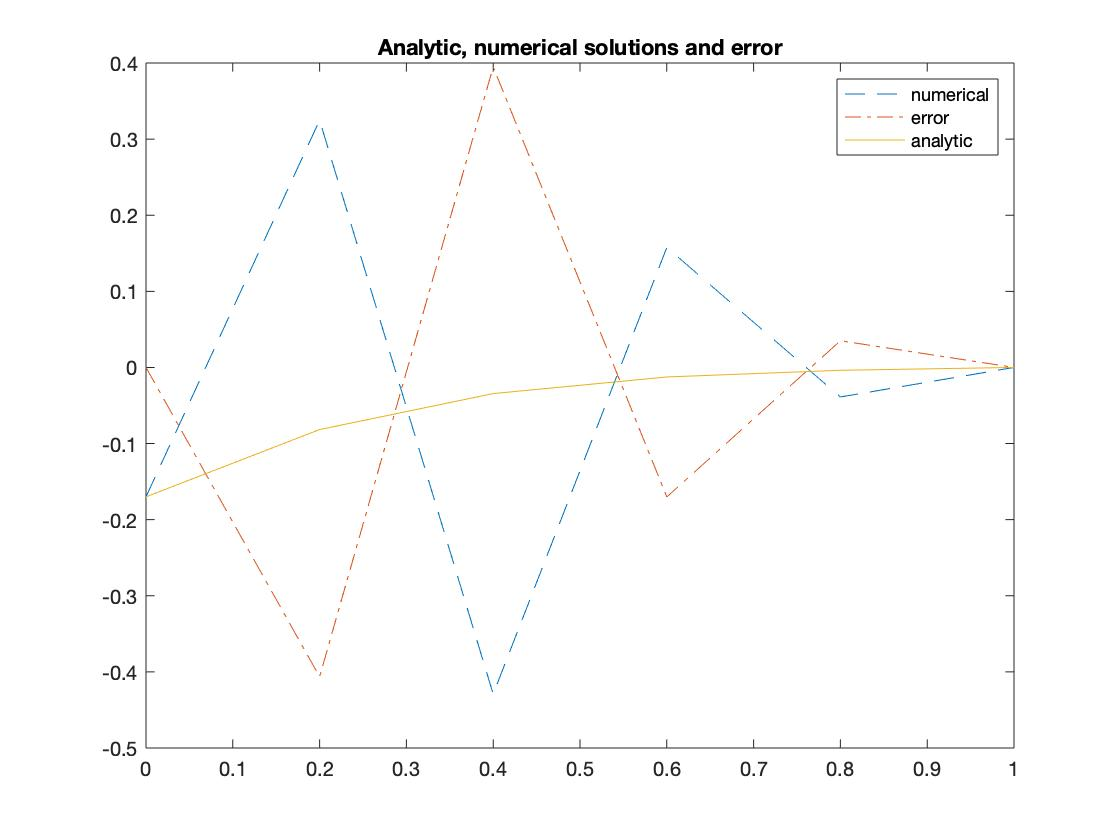
\includegraphics[width = \linewidth, height = 5cm]{Q2(5).jpg}
\caption{Figure 2.5: Analytic, numerical solution and error of scheme 2 at t = 0.1}
\label{Q2(5)}
\end{subfigure}
\begin{subfigure}{0.5\textwidth}
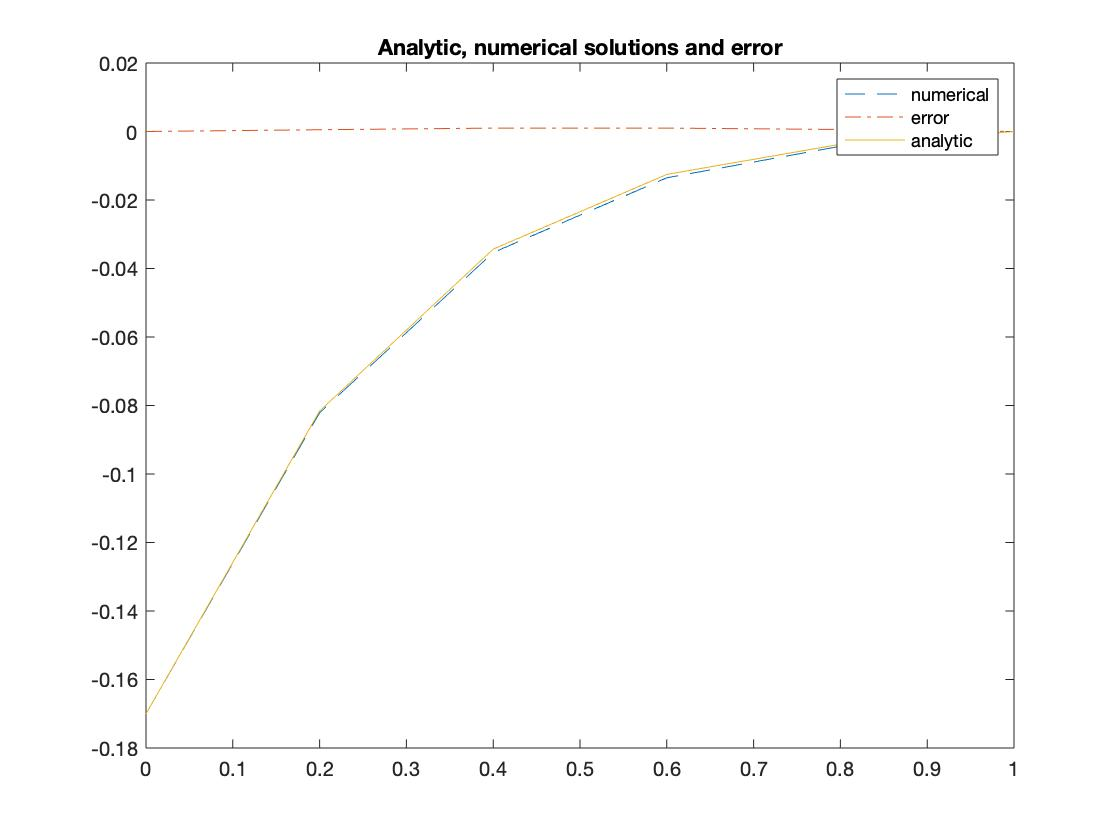
\includegraphics[width = \linewidth, height = 5cm]{Q2(6).jpg}
\caption{Figure 2.6: Analytic, numerical solution and error of scheme 3 at t = 0.1}
\label{Q2(6)}
\end{subfigure}
\end{figure}
\begin{table}[H]
\begin{tabular}{|c|c|c|c|c|c|c|c|}
\hline 
• & u1 & e1 & u2 & e2 & u3 & e3 & analytic \\ 
\hline 
x = 0 & -0.1700 & 0.0000 & -0.1700 & 0.0000 & -0.1700 & 0.0000 & -0.1700 \\ 
\hline 
x = h & -0.0798 & -0.0018 & 0.3248 & -0.4064 & -0.0821 & 0.0005 & -0.0816 \\ 
\hline 
x = 2h & -0.0322 & -0.0022 & -0.4292 & 0.3949 & -0.0353 & 0.0010 & -0.0343 \\ 
\hline 
x = 3h & -0.0094 & -0.0031 & 0.1576 & -0.1701 & -0.0135 & 0.0010 & -0.0125 \\ 
\hline 
 x = 4h & -0.0024 & -0.0013 & -0.0388 & 0.0351 & -0.0043& 0.0006 & -0.0037 \\ 
\hline 
x = 1 & 0.0000 & 0.0000 & 0.0000 & 0.0000 & 0.0000 & 0.0000 & 0.0000 \\ 
\hline 
\end{tabular} 
\caption{Table 1: analytic, numerical solutions and errors}
\label{T1}
\end{table}
\item
A few more plots were made by considering different values of $\nu$ and $\rho$. 
\item
Firstly, we analyze the stability of each scheme. A more precise definition of stability is that the norm of 
$\underline{u}^m$ is uniformly bounded for all m. We define the Fourier Transform(FT) of a series: $\hat{u}^m = \sum_{n\in \mathbb{Z}} e^{-in\theta} u_{n}^{m}$. Then by Parseval's theorem, Fourier Transform preserves the norm. 
In scheme 1 and 3, after taking FT of the whole equation, we obtain equations of the form: $\underline{u}^{m+1} = H(\theta)\underline{u}^{m}$. And clearly we need $\|H(\theta)\| \leqslant 1, \forall\ |\theta| \leqslant \pi$.\\
Specifically, in scheme 1 we have $H(\theta) = 1-4\nu\sin^2(\frac{\theta}{2})$ and in scheme 3 we have $$H(\theta) = 1-\frac{4\nu\sin^2{\frac{\theta}{2}}}{1+4\nu\rho\sin^2{\frac{\theta}{2}}}$$.\\
Therefore, 
For scheme 1 to be stable, we need $\nu \leqslant \frac{1}{2}$.
For scheme 3 to be stable, we need $\nu \leqslant \frac{1}{2(1-2\rho)}$.\\
Scheme 2 is different as we need to solve a difference equation of second order and make sure both of its roots have absolute value $\leqslant 1$. The two roots are $$-4\nu\sin^2(\frac{\theta}{2})\pm \sqrt{16\nu^2\sin^4(\frac{\theta}{2})+1}$$. And the minus root has an absolute value greater than 1 when $\sin(\frac{\theta}{2}) = 1$ for all positive $\nu$. Consequently, the scheme is not stable for all positive $\nu$, as we can see from \ref{Q2(2)}\\

The order of each scheme is calculated by Taylor expansion about about $u(nh,mk)$. The we consider the coefficient of leading order term. \\Scheme 2 has order 4 for any values of $\nu$. \\Since the coefficient of $h^4$ is $\frac{\nu(6\nu-1)}{12}$, scheme 1 has order 4 unless $\nu = \frac{1}{6}$, at which value the order is 6. Similarly, since the coefficient is $\frac{\nu((6(1-2\rho))\nu-1)}{12}$, scheme 3 has order 4 unless $\nu = \frac{1}{6(1-2\rho)}$, at which the order is 6 again.\\

Particularly, in scheme 3 we have the additional parameter $\rho$. From the previous stability analysis, if $\rho = 1/2$, this scheme is stable for all positive $\nu$. However, the order of accuracy cannot be higher than $h^4$ as $\nu$ is supposed to be a bounded positive constant. With $\rho = 1/2$, if we fix $k = \mu$ instead, then the stability is preserved for all positive $\mu$ as $\mu = h\nu$. We cannot gain the same accuracy as the order is dropped to 3, unless when $$\frac{\mu(\mu^2-\frac{1}{4})}{6} = 0$$, i.e. $\mu = 1/2$ when the order is 4.

\item
The 3rd scheme is the most suitable. Since Scheme 2 is unstable, we exclude it first. The order of scheme 1 and 3 are the same but 3 has better stability with specific parameters. Therefore, we choose scheme 3 with appropriate parameters. The Courant number should be large enough that the time step is not too small, and such that a large time can be reached within a manageable number of iterations. Therefore, we choose $v = 100$ and thus $\rho = \frac{1}{2}*(1-\frac{1}{6}*0.01)$ to maximize the order. 
The choice of N is relevant to the cost of computation. The computational cost is of order $\mathcal{O}((M-1)*(N-1))$. In each iteration, we solve the linear system $$L\underline{u}^{m+1}=R(\underline{u}^m+\underline{c})$$ with L being a band matrix of bandwidth 1. Therefore the computational cost is $\mathcal{O}(N-1)$. Therefore, we obtain the order of cost as claimed.
Then, if we choose t = 100 and N = 100. The total operation count is of order $\mathcal{O}(10^4)$, which is manageable by the computer. \\
We can see in the final figure that the error is indeed small as expected.
\begin{figure}[H]
\center
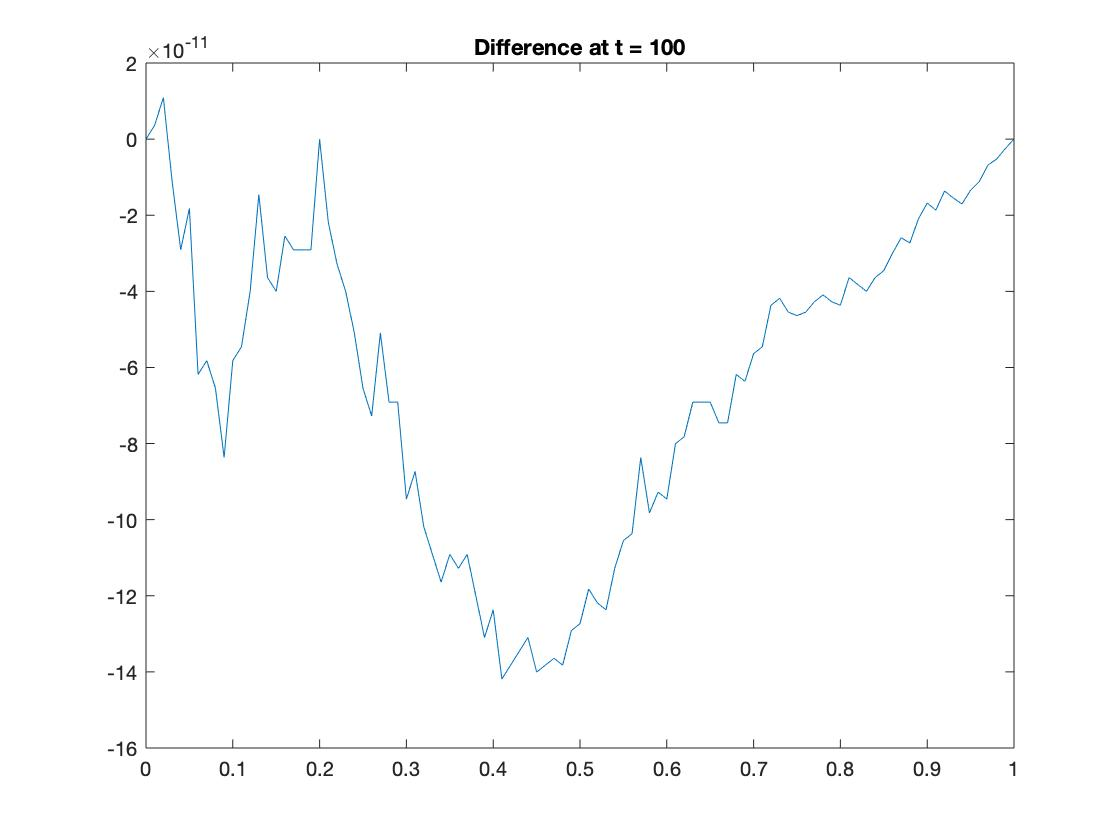
\includegraphics[width = 0.9\linewidth, height =8cm]{last.jpg}
\caption{Figure 2.7: Difference between the numerical solution of scheme 3 with parameters as suggested at t = 100}
\end{figure}
\end{enumerate}
\appendix
\section{Codes}
\subsection{P1}
\label{P1}
\lstinputlisting{Q1.m}
\newpage
\subsection{P2}
\label{P2}
\lstinputlisting{Q2.m}
\end{document}